\begin{frame}
	\frametitle{Redes neurais de pulso (RNP)}
	
	
	\only<1>{
		\framesubtitle{Características}
		\begin{itemize}
			\item funciona segundo limiares de ativação.
			\item redes esparsas (baixa ativação sináptica).
			\item uso de pulsos em vez de valores contínuos.
			\item processamento orientado ao tempo \cite{10242251}.
			\item tolerantes a ruídos (atuam como um filtro passa baixa).
			\item não um simulação de um-para-um como o neurônio Hodgkin-Huxley. \cite{gerstner2014neuronal} ou outros \cite{jones2020single}.
		\end{itemize}
	}
	
	\only<2>{
		\framesubtitle{\textit{Leaky Integrate and Fire Neurons} (LIF)}
		\begin{columns}
			\column{.5\linewidth}
				\begin{itemize}
					\item se assemelha com circuitos Resistor-Capacitor.
					\item os pulsos são representados como \textbf{uns} dispersamente distribuídos em uma sequência de \textbf{zeros}
					\item simples, mais eficientes e atualmente generalizam melhor para a maioria dos problemas \cite{dan_goodman_2022_7044500}.
				\end{itemize}
			\column{.5\linewidth}
			
			\begin{figure}[h]
				\centering
				\caption[Modelo RC]{O modelo RC}
				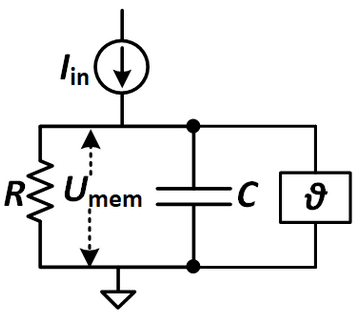
\includegraphics[width=.5\linewidth]{../monography/images/rcmodel}
				\label{fig:rcmodel}
			\end{figure}
		\end{columns}
	}
	\only<3>{
		\framesubtitle{\textit{Leaky Integrate and Fire Neurons} (LIF)}
		\par Gráfico do LIF simulado completo.
		\begin{figure}[H]
			\centering
			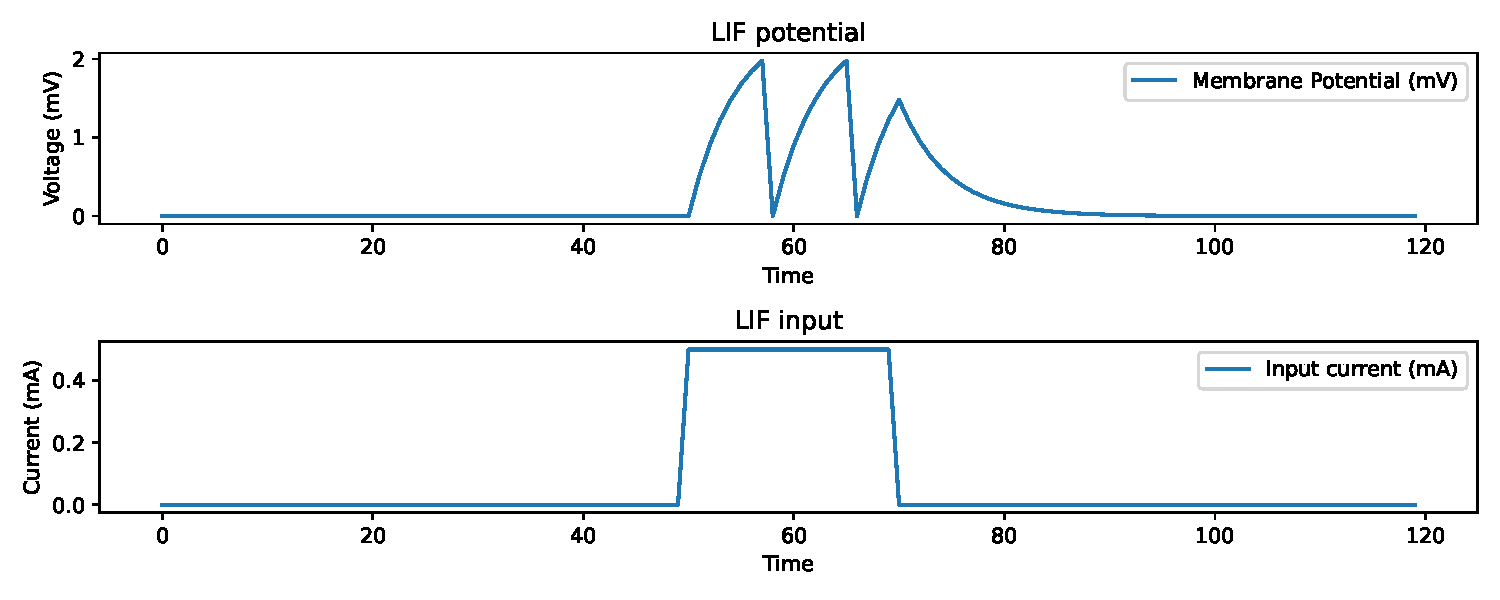
\includegraphics[width=.8\linewidth]{../monography/images/membranePotentialFull}
			\label{fig:membranepotentialfull}
		\end{figure}
	}
	\only<4>{
		\framesubtitle{Esparsidade}
		\par Atividade dispersa de uma RNP: O eixo horizontal representa o momento no qual os dados estão sendo processados e o vertical representa o número do neurônio (índice) na RNP. Note que, na maior parte do tempo, muito poucos neurônios são ativados.
		\begin{figure}[h]
			\centering
			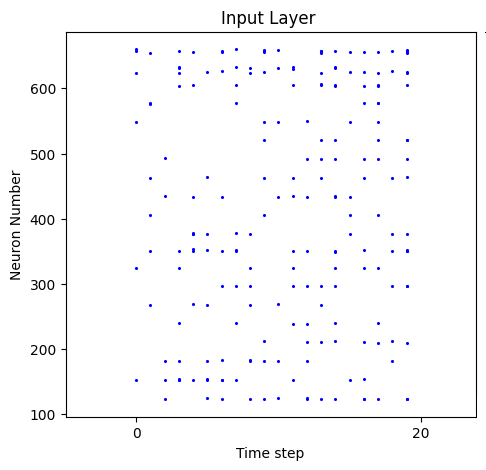
\includegraphics[width=.4\linewidth]{../monography/images/sparsity}
			\label{fig:sparsity}
		\end{figure}
	}
	
	\only<5>{
		\framesubtitle{Treinamento}
		\begin{itemize}
			\item \textbf{Plasticidade Dependente do Tempo de Pulsos (STDP)}: Se um neurônio pré-sináptico dispara \textbf{antes} do pós-sináptico, há um fortalecimento na conexão, mas se o neurônio pós-sináptico disparar antes, então há um enfraquecimento.
			\item \textbf{Descida de Gradiente Emprestada}: Aproxima a função de passo usando outra função matemática, que é diferenciável (como uma sigmoide), para treinar a rede. Essas aproximações são usadas apenas na fase de \textit{backpropagation}, enquanto mantêm a função de passo na fase do \textit{feed-forward}.
			\item \textbf{Algoritmos Evolutivos}: Usam a seleção dos mais aptos ao longo de muitas gerações de redes.
			\item \textbf{Reservatório/Computação Dinâmica}: \textbf{Redes de estado de eco} ou \textbf{Máquinas de estado líquido}, respectivamente.
		\end{itemize}
	}	
\end{frame}